\documentclass[11pt]{article}
\usepackage{amsmath, amssymb}
% \usepackage{natbib}
\usepackage{geometry}
\usepackage{float}
\usepackage[colorlinks=true, linkcolor=blue, citecolor=blue, urlcolor=blue]{hyperref}
\usepackage{setspace}
\usepackage{booktabs}
\usepackage{graphicx}
\usepackage{apacite}
\usepackage{natbib}
\usepackage{siunitx}
\usepackage{empheq}

\bibliographystyle{apacite}

\geometry{margin=1in}

\setstretch{1.2}
\title{Trade Tariffs and Exchange Rates: Revisiting Conventional Wisdom in a Three-Country Framework}


\author{
Jason Lu\thanks{International Monetary Fund, Research Department. Email: {\tt jlu2@imf.org}} 
\and 
Dimitre Milkov\thanks{International Monetary Fund, Research Department. Email: {\tt dmilkov@imf.org}}
}

\date{First draft: November 10, 2025 \\ This version: \today}

\begin{document}
\maketitle

\section*{Three-Country, Two-Sector, One-Factor Model}

\subsection*{Basic model setup}

We consider a static three-country, two-sector, one-factor (3c2s1f) model. 
Countries are indexed by $i \in \{A,B,C\}$, and goods by 
$g \in \{T_A, T_B, T_C, N\}$, where $T_i$ denotes the tradable good produced only in country $i$, and $N$ is a non-tradable good consumed exclusively domestically. Labor is the only factor of production and is immobile across countries. Without loss of generality, we normalize the domestic-currency price of each tradable variety to one:
\[
P_{T_i} \equiv 1, \qquad i \in \{A,B,C\}.
\]

\paragraph{Technology.}
Each country produces one distinct tradable good and one non-tradable good using linear technologies:
\begin{equation}
Y_{T_i} = A_{T_i} L_{T_i}, 
\qquad 
Y_{N_i} = A_{N_i} L_{N_i}, 
\qquad 
L_{T_i} + L_{N_i} = L_i,
\end{equation}
where $A_{T_i}$ and $A_{N_i}$ denote sectoral productivities, and $L_i$ is the labor endowment in country $i$.

\paragraph{Equilibrium wages.}
Under perfect competition and linear production technologies, wages satisfy
\begin{equation}
w_i = A_{T_i} = P_{N_i} A_{N_i}.
\label{eq:wage}
\end{equation}
This simplifies to
\[
w_i = A_{T_i}, 
\qquad 
P_{N_i} = \frac{A_{T_i}}{A_{N_i}}.
\]
Thus equilibrium wages and non-tradable prices are:
\[
w_{i,T} = A_{T_i}, 
\qquad 
w_{i,N} = P_{N_i} A_{N_i} = A_{T_i}, 
\qquad 
w_{i,T} = w_{i,N} = w_i.
\]

\paragraph{Household budget constraint.}
Let $C_{T_i i}$ denote country $i$’s consumption of its own tradable good, 
and $C_{T_j i}$ its consumption of the tradable good produced in country $j \neq i$. 
Let $e_{ij}$ denote the nominal exchange rate defined as units of country $i$’s tradable good per unit of country $j$’s tradable good. 
The household budget constraint in units of country $i$’s currency becomes
\begin{equation}
w_i L_i
\;=\;
C_{T_i i}
\;+\;
\sum_{\substack{j \in \{A,B,C\}\\ j \neq i}}
\big( e_{ij} \big)\, C_{T_j i}
\;+\;
P_{N_i}\, C_{N_i},
\qquad i \in \{A,B,C\}.
\end{equation}
Exchange rates satisfy $e_{ij}=1/e_{ji}$ and $e_{ij}=e_{ik}e_{kj}$ for all $i,j,k$.

\paragraph{Price level.}
Under Cobb--Douglas preferences, the price level in country $i$ is the minimum
expenditure required to achieve one unit of utility. The corresponding
unit-expenditure function is a geometric mean of consumer prices. In logs,
the price level is therefore
\begin{equation}
\log P_i
=
\sum_{j \in \{A,B,C\}} 
\alpha_{T_j}\, \log e_{ij}
\;+\;
\left(1 - \sum_{j \in \{A,B,C\}} \alpha_{T_j}\right)
\log P_{N_i},
\qquad i \in \{A,B,C\}.
\label{eq:price_level}
\end{equation}

\paragraph{Real exchange rate.} The bilateral real exchange rate between countries $i$ and $j$ is defined as the relative price of the consumption bundle in $j$ expressed in units of country $i$’s currency:
\begin{equation}
q_{ij} \equiv \frac{e_{ij} P_j}{P_i}, \qquad i,j \in \{A,B,C\}.
\label{eq:rer_bilateral}
\end{equation}

\paragraph{Terms of trade.} Country $i$'s terms of trade are defined as the ratio of its export price to its import price index. With producer prices normalized to one and consumer import prices $e_{ij}$ for $j\neq i$, the import price index consistent with Cobb--Douglas preferences is the geometric mean
\[
P^M_i = \prod_{j\neq i} e_{ij}^{\alpha_{T_j}}.
\]
Hence the terms of trade are
\begin{equation}
\mathrm{TOT}_i 
= \frac{1}{\prod_{j\neq i} e_{ij}^{\alpha_{T_j}}}, 
\qquad i\in\{A,B,C\}.
\label{eq:tot_notariffs}
\end{equation}


\paragraph{Household demand.}
Let the Cobb--Douglas expenditure shares on the three differentiated tradables be 
$\alpha_{T_A}, \alpha_{T_B}, \alpha_{T_C} \in (0,1)$ with 
$\alpha_{T_A} + \alpha_{T_B} + \alpha_{T_C} < 1$.
Preferences in each country $i$ are
\[
U_i 
= 
C_{T_A i}^{\alpha_{T_A}}\,
C_{T_B i}^{\alpha_{T_B}}\,
C_{T_C i}^{\alpha_{T_C}}\,
C_{N_i}^{\,1-\alpha_{T_A}-\alpha_{T_B}-\alpha_{T_C}},
\]
and the Cobb--Douglas coefficients are identical across countries.

The budget constraint in country $i$’s currency is
\[
w_i L_i
=
\sum_{j\in\{A,B,C\}}
\big( e_{ij} \big)\, C_{T_j i}
\;+\;
P_{N_i}\, C_{N_i},
\qquad i \in \{A,B,C\},
\]
where $e_{ii}=1$ and $e_{ij}$ is the nominal exchange rate between countries $i$ and $j$.
Cobb--Douglas structure implies expenditure shares equal the exponents:
\[
e_{ij}\, C_{T_j i}
=
\alpha_{T_j}\, w_i L_i,
\qquad
P_{N_i}\, C_{N_i}
=
\big(1-\alpha_{T_A}-\alpha_{T_B}-\alpha_{T_C}\big)\, w_i L_i.
\]

Hence the consumption quantities are
\begin{align}
C_{T_j i}
&=
\frac{\alpha_{T_j}\, w_i L_i}{e_{ij}},
\qquad j \in \{A,B,C\},
\\[4pt]
C_{N_i}
&=
\frac{\big(1-\alpha_{T_A}-\alpha_{T_B}-\alpha_{T_C}\big)\, w_i L_i}{P_{N_i}}.
\end{align}

\paragraph{Non-tradables market clearing.}
For each country $i \in \{A,B,C\}$,
\begin{equation}
Y_{N_i} = C_{N_i}.
\end{equation}
Using $Y_{N_i} = A_{N_i} L_{N_i}$, $P_{N_i} = w_i / A_{N_i}$, and Cobb--Douglas demand,
\begin{equation}
\frac{L_{N_i}}{L_i} 
= 1 - \alpha_{T_A} - \alpha_{T_B} - \alpha_{T_C},
\qquad
\frac{L_{T_i}}{L_i}
= \alpha_{T_A} + \alpha_{T_B} + \alpha_{T_C}.
\end{equation}

\paragraph{Tradables market clearing.}
For each tradable variety $T_i$ produced only in country $i$,
\begin{equation}
Y_{T_i}
=
\sum_{k \in \{A,B,C\}} C_{T_i k},
\qquad i \in \{A,B,C\}.
\end{equation}
Using $Y_{T_i} = A_{T_i} L_{T_i}$ and the Cobb--Douglas demands 
$e_{ki} C_{T_i k} = \alpha_{T_i} w_k L_k$ (with $e_{ii}=1$),
\begin{equation}
A_{T_i} L_{T_i}
=
\sum_{k \in \{A,B,C\}}
\frac{\alpha_{T_i}\, w_k L_k}{e_{ki}},
\qquad i \in \{A,B,C\}.
\label{eq:T_world_clearing_three_country}
\end{equation}
Here $e_{ki}$ denotes the nominal exchange rate expressed in units of country $k$’s currency per unit of country $i$’s currency, with the usual conditions $e_{ki} = 1/e_{ik}$ and $e_{ki} = e_{kj} e_{ji}$ for all $i,j,k$.

\paragraph{Trade balance.}
Let trade balances be measured in each country’s own currency. 
Country $i$’s exports of tradable $T_i$ to country $k$ are valued at 
$e_{ik}\, C_{T_i k}$, and its imports of tradable $T_j$ from country $j$ are valued at 
$e_{ij}\, C_{T_j i}$. 
The goods trade balance for country $i$ is therefore
\begin{equation}
\mathrm{TB}_i
=\sum_{\substack{k\in\{A,B,C\}\\ k\neq i}}
e_{ik}\, C_{T_i k}
\;-\;
\sum_{\substack{j\in\{A,B,C\}\\ j\neq i}}
e_{ij}\, C_{T_j i},
\qquad i\in\{A,B,C\}.
\label{eq:TB_three_country_def}
\end{equation}

Using Cobb--Douglas demand $e_{ij}\, C_{T_j i} = \alpha_{T_j}\, w_i L_i$ and $e_{ik}\, C_{T_i k} = \alpha_{T_i}\, w_k L_k$, we obtain
\begin{equation}
\mathrm{TB}_i
=
\sum_{\substack{k\neq i}}
\alpha_{T_i}\, w_k L_k
\;-\;
\sum_{\substack{j\neq i}}
\alpha_{T_j}\, w_i L_i.
\label{eq:TB_three_country_substituted}
\end{equation}
Balanced trade, $\mathrm{TB}_i=0$, then requires
\begin{equation}
\sum_{\substack{k\neq i}}
\alpha_{T_i}\, w_k L_k
\;=\;
\sum_{\substack{j\neq i}}
\alpha_{T_j}\, w_i L_i,
\qquad i\in\{A,B,C\}.
\label{eq:TB_three_country_condition}
\end{equation}

\paragraph{Equilibrium condition.}
With three countries and three tradables, Walras' Law implies that only 
two of the three trade-balance conditions in~\eqref{eq:TB_three_country_condition} are independent. 
Together with the normalization of tradable prices and the two independent bilateral exchange rates 
$\{e_{AB}, e_{AC}\}$ (with $e_{BC}=e_{BA}e_{AC}$), these conditions determine the 
equilibrium nominal exchange rates consistent with balanced trade across all three countries.

\begin{figure}[h]
    \centering
    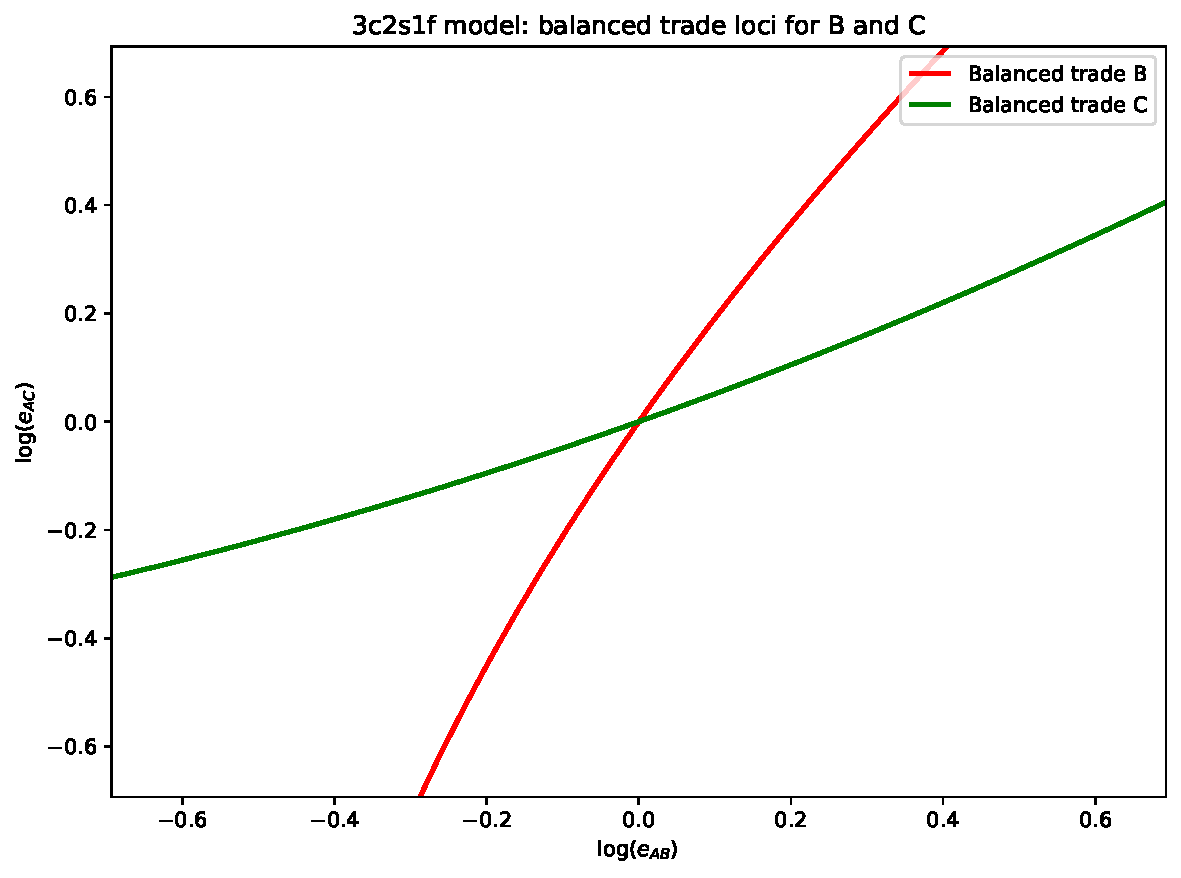
\includegraphics[width=0.8\textwidth]{3c2s1f_eq.pdf}
    \caption{3c2s1f model: trade balance loci in bilateral exchange rates.}
    \label{3c2s1f_eq}
\end{figure}

Figure~\ref{3c2s1f_eq} plots the sets of bilateral exchange rates 
$(e_{AB}, e_{AC})$ that satisfy the trade balance conditions for countries~B and~C
in the three--country, two--sector, one--factor model. The equilibrium occurs at the intersection of these two loci. 
The plot is generated for $A_{T_i}=A_{N_i}=1$, 
$\alpha_{T_A}=\alpha_{T_B}=\alpha_{T_C}=\alpha_N=1/4$, and normalized tradable 
prices $P_{T_i}=1$.

Due to the symmetry of the model with respect to countries B and C, 
the balanced trade loci for these two countries are reflections of each other 
across the line $y = x$. In particular, if we move along the red line above the intersection point, B has balanced trade, but A has a surplus while C a deficit.

\section*{Unilateral Tariffs}

We now introduce ad valorem tariffs levied by country~A on its imports of the 
two foreign tradable goods.  Let $\tau_B \ge 0$ denote the tariff applied to 
imports of $T_B$, and $\tau_C \ge 0$ the 
tariff applied to imports of $T_C$.

The tariffs raise the consumer prices of imported goods in A to
\[
(1+\tau_B)e_{AB} \quad\text{for imports of } T_B,
\qquad
(1+\tau_C)e_{AC} \quad\text{for imports of } T_C.
\]
Producers in countries~B and~C continue to receive the normalized domestic price of~1, 
so the wedges $\tau_B e_{AB}$ and $\tau_C e_{AC}$ represent tariff revenue.

Country~A’s household budget constraint becomes
\begin{equation}
w_A L_A + T_A^{\mathrm{rev}}
=
C_{T_A A}
+ (1+\tau_B)e_{AB}\, C_{T_B A}
+ (1+\tau_C)e_{AC}\, C_{T_C A}
+ P_{N_A}\, C_{N_A},
\end{equation}
where tariff revenue is
\begin{equation}
T_A^{\mathrm{rev}}
= \tau_B e_{AB}\, C_{T_B A}
+ \tau_C e_{AC}\, C_{T_C A},
\end{equation}
and is rebated lump-sum to households in~A.

Cobb--Douglas preferences imply that the value of expenditures on 
$(T_A, T_B, T_C, N_A)$ remains proportional to the shares 
$(\alpha_{T_A},\alpha_{T_B},\alpha_{T_C},\alpha_N)$, but the higher consumer 
prices $(1+\tau_B)e_{AB}$ and $(1+\tau_C)e_{AC}$ reduce the quantities of 
$T_B$ and $T_C$ imported by country~A.  Countries~B and~C do not impose tariffs 
and therefore retain the same budget constraints as in the free-trade benchmark. 

Solving for demand as a function of parameters, prices, exchange rates, and tariff rates, gives:

\paragraph{Demand in country~A:}
\begin{align}
C_{T_A A} &= \alpha_{T_A}\, I_A, \\[6pt]
C_{T_B A} &= \alpha_{T_B} \frac{I_A}{(1+\tau_B)e_{AB}}, \\[6pt]
C_{T_C A} &= \alpha_{T_C} \frac{I_A}{(1+\tau_C)e_{AC}}, \\[6pt]
C_{N_A}   &= \alpha_N \frac{I_A}{P_{N_A}}.
\end{align}

\paragraph{Demand in country~B:}
\begin{align}
C_{T_A B} &= \alpha_{T_A} \frac{w_B L_B}{e_{BA}}, \\[6pt]
C_{T_B B} &= \alpha_{T_B} w_B L_B, \\[6pt]
C_{T_C B} &= \alpha_{T_C} \frac{w_B L_B}{e_{BC}}, \\[6pt]
C_{N_B}   &= \alpha_N \frac{w_B L_B}{P_{N_B}}.
\end{align}

\paragraph{Demand in country~C:}
\begin{align}
C_{T_A C} &= \alpha_{T_A} \frac{w_C L_C}{e_{CA}}, \\[6pt]
C_{T_B C} &= \alpha_{T_B} \frac{w_C L_C}{e_{CB}}, \\[6pt]
C_{T_C C} &= \alpha_{T_C} w_C L_C, \\[6pt]
C_{N_C}   &= \alpha_N \frac{w_C L_C}{P_{N_C}}.
\end{align}

$I_A$ is given by
\begin{equation}
I_A
= \frac{w_A L_A}{
1
- \dfrac{\tau_B\, \alpha_{T_B}}{1+\tau_B}
- \dfrac{\tau_C\, \alpha_{T_C}}{1+\tau_C}
},
\end{equation}
and wages and the price of the nontradable are given by
\[
\begin{aligned}
w_i &= A_{T_i}, 
&\qquad 
P_{N_i} &= \frac{A_{T_i}}{A_{N_i}}.
\end{aligned}
\]



\paragraph{Market clearing and equilibrium.}
Tariffs in country~A do not affect domestic production.  
With linear technologies and competitive firms, producer prices remain 
$P_{T_i}=1$, so wages continue to satisfy $w_i = A_{T_i}$ and the 
nontradable prices $P_{N_i}=A_{T_i}/A_{N_i}$ are unchanged.  
Because the tariffs apply only to the consumer prices of $T_B$ and $T_C$ in~A, 
but not to the producer prices received abroad, the production side of the 
economy is unaffected and the sectoral labor allocations 
$(L_{T_i},L_{N_i})$ remain at their free-trade values.

Tariff revenue in~A is rebated lump-sum, raising household income but leaving 
Cobb--Douglas expenditure shares unchanged.  The only effect of the tariffs is 
therefore on the quantities of $T_B$ and $T_C$ that A imports through the 
higher consumer prices $(1+\tau_B)e_{AB}$ and $(1+\tau_C)e_{AC}$. With three countries, the trade balance equations are unchanged. Simultaneous trade balance determine the equilibrium values of $e_{AB}$ and $e_{AC}$.

\subsection*{Uniform tariffs.} 
We first investigate what happens to equilibrium exchange rates when country A imposes uniform tariffs on exports from country B and country C.

\begin{figure}[H]
    \centering
    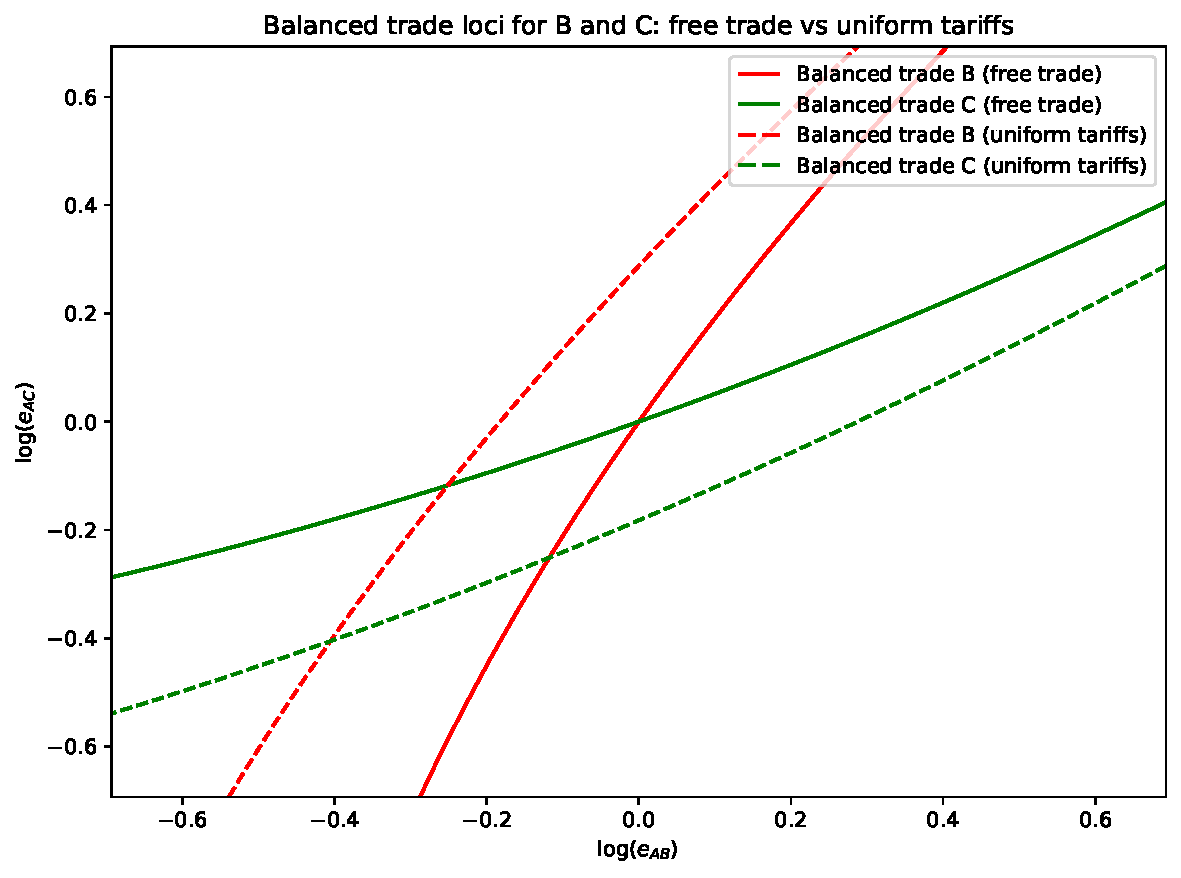
\includegraphics[width=0.8\textwidth]{3c2s1f_eq_uniform_tariffs.pdf}
    \caption{3c2s1f model with equal tariffs: trade balance loci.}
    \label{fig:3c2s1f_eq_uniform_tariffs}
\end{figure}

Figure~\ref{fig:3c2s1f_eq_uniform_tariffs} plots the trade-balance loci for countries~A and~B
in the three-country model, comparing the free-trade case 
($\tau_B=\tau_C=0$, solid lines) with a uniform tariff imposed by $A$
($\tau_B=\tau_C=1$, dashed lines).  
The calibration sets $A_{T_i}=A_{N_i}=1$ and $\alpha_{T_i}=\alpha_N=1/4$.  

Equilibrium occurs at the intersection of the $TB_B = 0$ and $TB_C = 0$ curves. 
Introducing equal tariffs in country~A shifts both loci outward relative to the 
$y = x$ line and leads to an appreciation of country~A’s currency with respect 
to both countries~B and~C. In particular, given the symmetry of the calibration 
across countries and the uniform tariff applied to imports from both B and~C, 
country~A’s currency must appreciate by the same amount relative to the 
currencies of B and~C.


\subsection*{Single–country tariff}

We next consider the case where country~A imposes a tariff only on imports 
from country~B, leaving imports from country~C untaxed.

\begin{figure}[H]
    \centering
    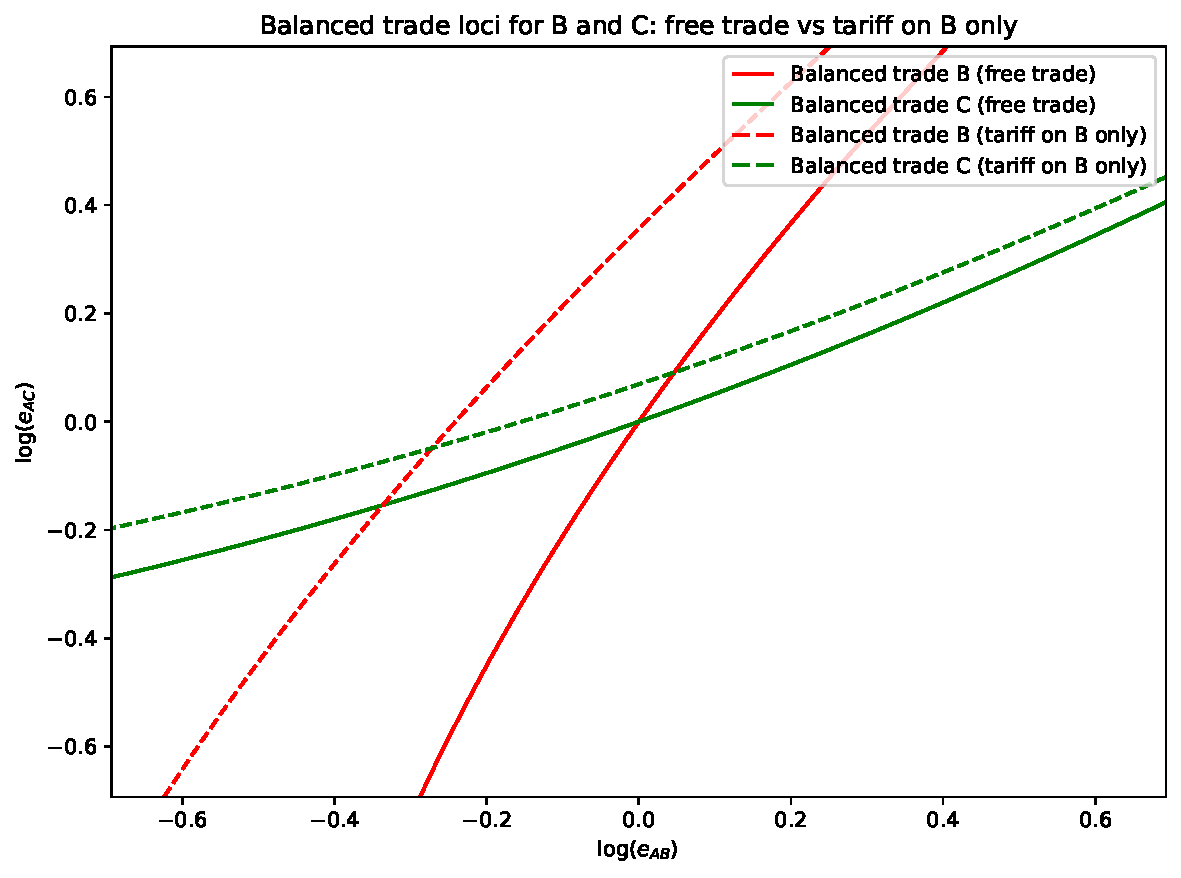
\includegraphics[width=0.8\textwidth]{3c2s1f_eq_single_tariff.pdf}
    \caption{3c2s1f model with a tariff on imports from B only: trade balance loci.}
    \label{fig:3c2s1f_eq_single_tariff}
\end{figure}

Figure~\ref{fig:3c2s1f_eq_single_tariff} plots the balanced-trade loci for countries~B 
and~C in the three–country model, comparing the free–trade case 
($\tau_B=\tau_C=0$, solid lines) with a tariff imposed only on country~B 
($\tau_B=1,\ \tau_C=0$, dashed lines).  

Introducing a tariff on imports from~B shifts country~B’s balanced-trade locus 
outward from the $y = x$ line, while shifting country~C’s balanced-trade locus 
inward. The effect on $e_{AB}$ is therefore unambiguously negative, whereas the 
net effect on $e_{AC}$ is ambiguous.

\paragraph{Ambiguous effect on the bilateral exchange rate $e_{AC}$.}

When country~A imposes a tariff on imports from country~B, the resulting
general–equilibrium effects on the bilateral exchange rate $e_{AC}$ are
inherently ambiguous. The tariff triggers two opposing forces that operate
through changes in the pattern of trade flows.

\emph{First}, the tariff induces a \textbf{trade–diversion effect}:
imports into~A shift away from~B toward alternative suppliers, most
prominently country~C. As A reallocates expenditure toward goods produced
by~C, the demand for C's exports rises, improving its trade balance. In
equilibrium, this tends to generate an \textbf{appreciation of country~C's
currency}, i.e.
\[
e_{AC} \;\downarrow,
\]
since fewer units of A's currency are required to purchase one unit of
C's currency.

\emph{Second}, the tariff also induces a \textbf{trade–redirection effect}:
as B loses access to A's market, it reallocates exports toward C. From
the perspective of country~C, this represents an increase in imports from~B,
which tends to deteriorate C's trade balance. To restore external balance,
the relative price of C's goods must fall, generating a
\textbf{depreciation of C's currency}, i.e.
\[
e_{AC} \;\uparrow.
\]

The net movement in $e_{AC}$ is therefore determined by the relative
magnitudes of these two forces. If the improvement in C's exports to~A
(trade diversion) dominates the increase in imports from~B (trade
redirection), then C experiences an appreciation. Conversely, if the
import increase dominates, C must depreciate.

\paragraph{When does the appreciation of country C dominate?}

Although the sign of the exchange–rate response is theoretically
indeterminate, economic intuition points to a set of circumstances under
which the appreciation of~C is more likely to dominate:

\begin{itemize}
    \item \textbf{High substitutability between B's and C's goods in A's
    market.} When goods from~B and~C are close substitutes, a tariff on~B
    induces a large reallocation of A's demand toward~C, strengthening C's
    trade balance.

    \item \textbf{Large expenditure share of C's goods in A's consumption.}
    If C already plays an important role as a supplier to~A, even small
    changes in relative prices generate sizable shifts in demand toward~C.

    \item \textbf{Country C is relatively productive or competitive in
    tradables.} Higher productivity or lower marginal cost enables~C to
    expand exports to~A without requiring a significant deterioration in
    its terms of trade, magnifying the trade–diversion channel.

    \item \textbf{Baseline imports of C from B are small.}
    If country~C initially relies only minimally on B as a supplier, the
    redirection of B’s exports toward~C generates only a modest increase in
    C’s imports, weakening the depreciation channel.

    \item \textbf{The tariff imposed by A is sufficiently large.}
    Large tariff shocks generate large reallocations of A's import demand
    away from~B and toward~C, amplifying the appreciation channel.

\end{itemize}

In combination, these conditions make it more likely that the positive
trade–balance effect associated with increased exports from~C to~A outweighs
the negative effect of increased imports from~B, resulting in a net
\textbf{appreciation} of C's currency relative to A.

\paragraph{Alternative demand specifications with non-symmetric elasticities.}

The symmetric CES Armington aggregator imposes a single elasticity of
substitution $\sigma$ across all traded varieties. This implies identical
substitutability among all foreign suppliers, identical substitutability
between domestic and foreign sources, and full symmetry across importers.
Empirically, however, these restrictions are highly unrealistic. For
instance, U.S.\ imports from China and Vietnam are extremely close
substitutes, while U.S.\ domestic products are far less substitutable
with low-cost Asian imports, and Vietnam's ability to substitute between
Chinese and U.S.\ goods is limited. Such asymmetries cannot be reproduced
within a one-parameter CES system.

This section describes several alternative demand specifications that
permit non-symmetric elasticities while remaining tractable.

\paragraph{(i) Two-level nested CES.}

Tradable consumption in country $A$ may be written as
\begin{align}
C_A
&=
\left[
  \gamma_A \, C_{A,A}^{\frac{\rho-1}{\rho}}
  +
  (1-\gamma_A)
  \, M_A^{\frac{\rho-1}{\rho}}
\right]^{\frac{\rho}{\rho-1}},
\\[0.5em]
M_A
&=
\left[
  \beta_A \, C_{A,B}^{\frac{\eta-1}{\eta}}
  +
  (1-\beta_A) \, C_{A,C}^{\frac{\eta-1}{\eta}}
\right]^{\frac{\eta}{\eta-1}},
\end{align}
where $\rho$ governs the elasticity of substitution between domestic and
imported goods, and $\eta$ governs the elasticity among foreign suppliers
(e.g.\ China and Vietnam). Choosing $\eta \gg \rho$ allows for realistic
situations in which Chinese and Vietnamese exports are close substitutes
for U.S.\ consumers, while domestic products are imperfect substitutes for
either foreign variety.

\paragraph{(ii) Importer-specific CES.}

For importer $k \in \{A,B,C\}$, tradable consumption satisfies
\[
C_k
=
\left(
  \sum_{i \in \{A,B,C\}}
    \alpha_{k,i}
    C_{k,i}^{\frac{\sigma_k - 1}{\sigma_k}}
\right)^{\frac{\sigma_k}{\sigma_k - 1}}.
\]

The elasticity of substitution $\sigma_k$ is now importer-specific.
For example, one may set
\[
\sigma_A \gg \sigma_B \approx \sigma_C,
\]
to reflect that U.S.\ consumers view Chinese and Vietnamese goods as close
substitutes, while Vietnam and China do not substitute strongly between
each other's goods.

\paragraph{(iii) Translog demand system.}

Let $p_i$ denote the consumer price of variety $i$ and $x$ total
expenditure. A translog expenditure function is
\[
\ln x
=
\alpha_0
+
\sum_i \alpha_i \ln p_i
+
\tfrac{1}{2}
\sum_i \sum_j \gamma_{ij} \ln p_i \ln p_j,
\]
with $\gamma_{ij} = \gamma_{ji}$ unrestricted (aside from integrability).
The Hicksian substitution elasticities are given by
\[
\sigma_{ij}
=
\frac{s_i s_j}{\gamma_{ij}},
\]
where $s_i$ is the expenditure share. This system permits a full matrix of
pair-specific elasticities $\sigma_{ij}$ that can differ across both goods
and directions, thereby capturing, for example, strong substitution
between Chinese and Vietnamese goods for U.S.\ consumers, but weak
substitution between Chinese and U.S.\ goods for Vietnamese consumers.

\paragraph{(iv) Almost Ideal Demand System (AIDS).}

Budget shares satisfy
\[
s_i
=
\alpha_i
+
\sum_j \gamma_{ij} \ln p_j
+
\beta_i \ln\!\left(\frac{x}{P}\right),
\]
where $P$ is a translog price index.
Elasticities of substitution are
\[
\sigma_{ij}
=
\delta_{ij}
-
\frac{\gamma_{ij} + \beta_i \beta_j \ln(x/P)}
      {s_i s_j},
\]
allowing rich heterogeneity across pairs $(i,j)$.

\paragraph{(v) CES with taste/quality shifters.}

Let $\theta_{k,i}$ denote country $k$'s taste weight for variety $i$.
Then
\[
C_k
=
\left(
  \sum_i
    \theta_{k,i}
    C_{k,i}^{\frac{\sigma - 1}{\sigma}}
\right)^{\frac{\sigma}{\sigma - 1}}.
\]

By choosing $\theta_{k,i}$ appropriately, one can mimic low substitution
for certain pairs even if $\sigma$ is common, because effective prices are
scaled by the taste parameters. This retains CES tractability while
allowing limited asymmetry in bilateral substitution patterns.



\section*{Multiateral Tariffs}

We now introduce a general system of ad valorem taxes on tradable consumption, 
levied by each country on its purchases of tradable goods produced at home or abroad. 
Let $\tau_{ij} \ge 0$ denote the tax that country~$i$ applies to consumption of 
tradable $T_j$ produced in country~$j$. The case $i \neq j$ corresponds to an 
import tariff, while the case $i=j$ corresponds to a general consumption tax on 
the home tradable good.

These taxes raise the consumer prices of tradable goods in country~$i$ to
\[
(1+\tau_{ij})\, e_{ij}
\quad\text{for consumption of } T_j \text{ in country } i,
\]
where $e_{ij}$ is the nominal exchange rate between countries $i$ and $j$, defined as 
the price of one unit of currency~$j$ in units of currency~$i$, and we normalize 
$e_{ii}=1$. Producers in country~$j$ continue to receive the normalized domestic price 
of~1, so the wedge $\tau_{ij} e_{ij}$ represents tax revenue for country~$i$.

Country~$i$'s household budget constraint becomes
\begin{equation}
w_i L_i + T_i^{\mathrm{rev}}
=
\sum_{j} (1+\tau_{ij})\, e_{ij}\, C_{T_j i}
+ P_{N_i}\, C_{N_i},
\end{equation}
where tax revenue is
\begin{equation}
T_i^{\mathrm{rev}}
= \sum_{j} \tau_{ij}\, e_{ij}\, C_{T_j i},
\end{equation}
and is rebated lump sum to households in country~$i$.

\paragraph{Price level under multilateral tariffs.}
With ad valorem taxes $\tau_{ij}$ applied by country $i$ to consumption of tradable good $T_j$, the consumer price of $T_j$ in $i$ is $(1+\tau_{ij}) e_{ij}$. Under Cobb--Douglas preferences, the unit-expenditure function is the share-weighted geometric mean of consumer prices. Hence the (log) price level in country $i$ is
\begin{equation}
\log P_i 
= 
\sum_{j\in\{A,B,C\}} 
\alpha_{T_j}\, \log\!\big[(1+\tau_{ij}) e_{ij}\big]
\;+\;
\Bigl(1 - \sum_{j\in\{A,B,C\}} \alpha_{T_j}\Bigr)\, \log P_{N_i},
\qquad i\in\{A,B,C\}.
\label{eq:price_level_tariffs}
\end{equation}

\paragraph{Real exchange rate under multilateral tariffs.} 
The bilateral real exchange rate between countries $i$ and $j$ is defined as the relative price of country $j$’s consumption bundle expressed in units of country $i$’s currency,
\begin{equation}
q_{ij} \equiv \frac{e_{ij} P_j}{P_i}, \qquad i,j \in \{A,B,C\},
\label{eq:rer_tariffs}
\end{equation}
where $P_i$ and $P_j$ are the tariff-adjusted price levels.

% \paragraph{Terms of trade under multilateral tariffs.}
% Country $i$'s terms of trade are defined as the ratio of its export price to its import price index. 
% With producer prices normalized to one and consumer import prices equal to $(1+\tau_{ij}) e_{ij}$ for $j\neq i$, the import price index is the share-weighted geometric mean of these prices. 
% Hence the terms of trade for country $i$ are
% \begin{equation}
% \mathrm{TOT}_i
% =
% \frac{1}{
% \prod_{j \neq i}
% \left[(1+\tau_{ij})\, e_{ij}\right]^{\, \alpha_{T_j} / \sum_{k\neq i} \alpha_{T_k}}
% },
% \qquad i \in \{A,B,C\}.
% \label{eq:tot_tariffs}
% \end{equation}

% \paragraph{Log-linearized terms of trade.}
% Taking logs of the expression for the terms of trade under multilateral tariffs and using the first-order approximation $\ln(1+\tau_{ij}) \approx \tau_{ij}$, we obtain
% \begin{equation}
% \log \mathrm{TOT}_i
% \;\approx\;
% - \sum_{j\neq i} 
% \frac{\alpha_{T_j}}{\sum_{k\neq i} \alpha_{T_k}}
% \left[ \tau_{ij} + \log e_{ij} \right],
% \qquad i \in \{A,B,C\}.
% \label{eq:tot_log_lin}
% \end{equation}



\paragraph{Demand functions.}
Let $\alpha = (\alpha_{T_A},\alpha_{T_B},\alpha_{T_C})^\top$ collect the 
Cobb--Douglas shares on the three tradable goods and let 
$I = (I_A,I_B,I_C)^\top$ collect household disposable incomes in the three countries. 
Let
\begin{equation}
E = (e_{ij})_{i,j}, 
\qquad 
T = (\tau_{ij})_{i,j},
\end{equation}
denote the exchange rate and tax matrices, and let 
\begin{equation}
p_T = (P_{T_A},P_{T_B},P_{T_C})^\top
\end{equation}
stack producer prices of tradables.

Define the $3\times 3$ consumer price matrix for tradables as
\begin{equation}
P^{c}
=
\bigl[(\mathbf{1}\mathbf{1}^\top + T)\,\odot\,E\bigr]\,
\mathrm{diag}(p_T),
\end{equation}
so that each entry is
\begin{equation}
P^{c}_{ji} 
= (1+\tau_{ij})\, e_{ij}\, P_{T_j}.
\end{equation}

Cobb--Douglas tradable demands can then be written compactly as
\begin{equation}
C_T
=
\bigl(\alpha\, I^\top\bigr)
\,\oslash\,
P^{c},
\end{equation}
where $(\alpha\, I^\top)_{ji} = \alpha_{T_j} I_i$ and $\oslash$ denotes elementwise division. 
Thus, for each good $T_j$ consumed in each country $i$,
\begin{equation}
(C_T)_{ji}
=
\frac{\alpha_{T_j} I_i}{P^{c}_{ji}}
=
\frac{\alpha_{T_j} I_i}{(1+\tau_{ij})\, e_{ij}\, P_{T_j}}.
\end{equation}

If producer prices are normalized to one, $p_T \equiv \mathbf{1}$, then
\begin{equation}
P^{c}
=
(\mathbf{1}\mathbf{1}^\top + T)\,\odot\,E,
\end{equation}
and
\begin{equation}
C_T
=
\bigl(\alpha\, I^\top\bigr)\,\oslash\,
\bigl[(\mathbf{1}\mathbf{1}^\top + T)\,\odot\,E\bigr].
\end{equation}

Let factor incomes be $Y = (Y_A,Y_B,Y_C)^\top$ with $Y_i = w_i L_i$.
Tariff (or consumption tax) revenue in country $i$ is
\begin{equation}
T_i^{\mathrm{rev}}
=
\sum_{j} \tau_{ij}\, e_{ij}\, C_{T_j i},
\end{equation}
which, using the Cobb--Douglas demands, implies disposable income
\begin{equation}
I_i
=
\frac{Y_i}{
1 - \displaystyle\sum_{j} \alpha_{T_j}\, \frac{\tau_{ij}}{1+\tau_{ij}}
}.
\end{equation}

In matrix form, define the $3\times 3$ matrix $\Gamma = (\gamma_{ij})$ with
\begin{equation}
\gamma_{ij}
=
\alpha_{T_j}\, \frac{\tau_{ij}}{1+\tau_{ij}},
\end{equation}
so that tariff revenue can be written as $\Gamma I$ and disposable income satisfies
\begin{equation}
I = Y + \Gamma I
\quad\Rightarrow\quad
(\mathbf{I}_3 - \Gamma)\, I = Y
\quad\Rightarrow\quad
I = (\mathbf{I}_3 - \Gamma)^{-1} Y.
\end{equation}

\subsection*{Bilateral trade war}

We next investigate how equilibrium exchange rates respond when country~A 
imposes a tariff on imports from country~B and country~B retaliates with an 
equal tariff on imports from country~A.

\begin{figure}[H]
    \centering
    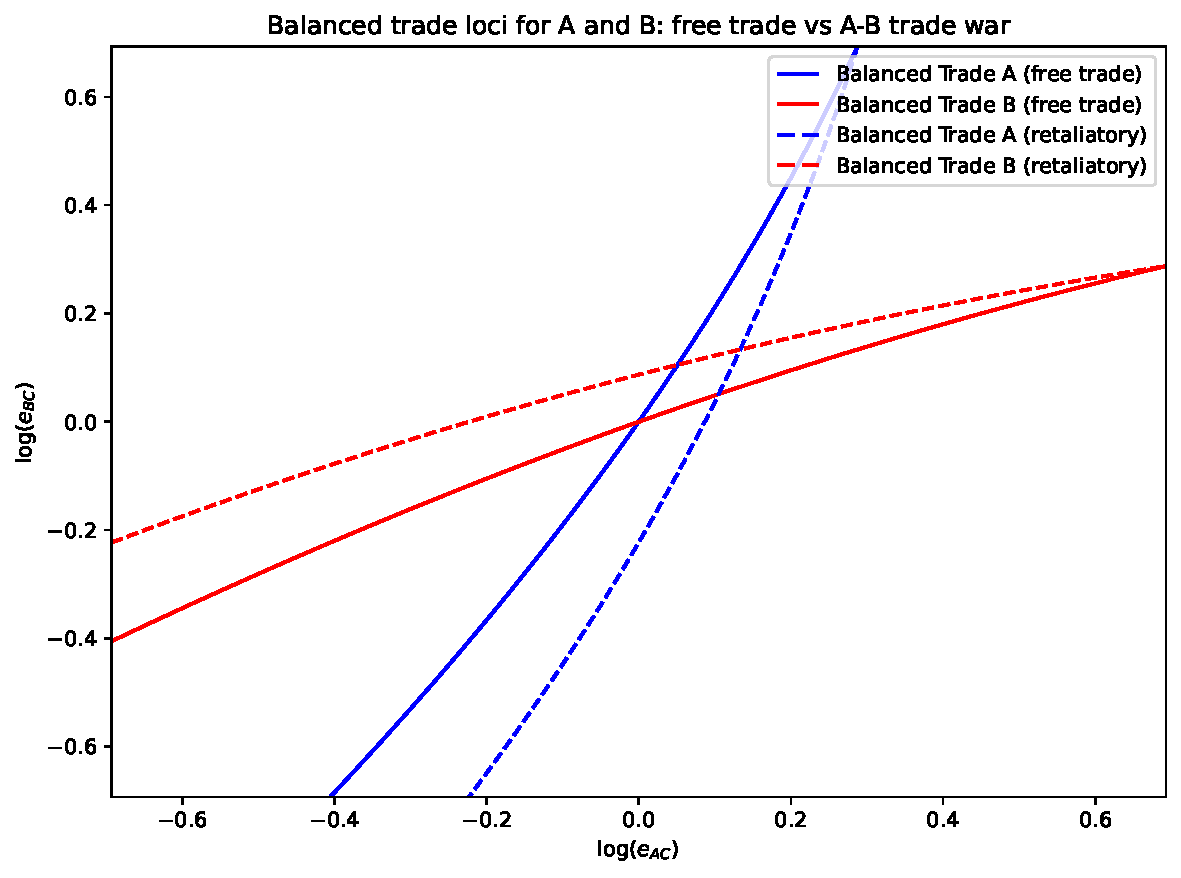
\includegraphics[width=0.8\textwidth]{3c2s1f_eq_trade_war.pdf}
    \caption{3c2s1f model with reciprocal tariffs between A and B: trade balance loci.}
    \label{fig:3c2s1f_eq_trade_war}
\end{figure}

Figure~\ref{fig:3c2s1f_eq_trade_war} plots the balanced-trade loci for 
countries~A and~B in the three-country model, comparing the free-trade case 
(solid lines) with a bilateral trade war in which 
$\tau_{AB} = \tau_{BA} = 1$ and all other tariff rates remain zero (dashed lines). 
The calibration sets $A_{T_i}=A_{N_i}=1$ and $\alpha_{T_i}=\alpha_N=1/4$.

Equilibrium occurs at the intersection of the $TB_A = 0$ and $TB_B = 0$ curves. 
The introduction of mutually imposed tariffs between A and~B shifts both 
countries’ balanced-trade loci outward in the $(e_{AC}, e_{BC})$ exchange-rate 
space. Because the tariff is bilateral rather than uniform, the symmetry that 
previously existed between countries~B and~C in the unilateral tariff case 
(now that A alone imposed tariffs) shifts to a symmetry between A and~B, which 
now impose tariffs on one another, while country~C remains distinct because it 
is not subject to any tariff by either country.


In general, the reciprocal tariffs generate offsetting pressures on the 
A--B bilateral exchange rate, which remains unchanged in the trade war. 
They do, however, alter each country’s effective expenditure on imports 
from~C. As a result, the new equilibrium requires a reallocation across all 
three trading relationships. This adjustment is achieved through a joint 
depreciation of the currencies of A and~B relative to the currency of~C.

\section*{CES Utility in the 3-Country Model}

In the baseline model, each country $i$ consumes a composite of
tradable goods $j \in \{A,B,C\}$ and a nontradable good $N$.
We now replace the Cobb--Douglas utility function with a CES utility function.

\subsection*{CES Preferences}

Let the consumption bundle in country $i$ be
\[
C_i = 
\left[
    \alpha_N^{1/\sigma} C_{iN}^{\frac{\sigma-1}{\sigma}}
    + \sum_{j \in T} \alpha_j^{1/\sigma} C_{ij}^{\frac{\sigma-1}{\sigma}}
\right]^{\frac{\sigma}{\sigma-1}},
\]
where:
\begin{itemize}
    \item $\sigma > 0$ is the elasticity of substitution across goods, 
    \item $\alpha_j > 0$ are taste parameters such that 
          $\alpha_N + \sum_{j \in T} \alpha_j = 1$,
    \item $T = \{A,B,C\}$ denotes the tradables set.
\end{itemize}

Let $P_{ij}$ denote the consumer price in country $i$ for good $j$.
For nontradables, $P_{iN}$ is the local nontradable price.

\subsection*{CES Price Index}

The corresponding CES price index in country $i$ is
\[
P_i = 
\left[
    \alpha_N^\sigma P_{iN}^{1-\sigma}
    + \sum_{j \in T} \alpha_j^\sigma P_{ij}^{1-\sigma}
\right]^{\frac{1}{1-\sigma}}.
\]

Define the CES denominator:
\[
D_i 
= 
\alpha_N^\sigma P_{iN}^{1-\sigma}
+ \sum_{j \in T} \alpha_j^\sigma P_{ij}^{1-\sigma}.
\]

\subsection*{CES Demand System}

Given nominal income $I_i$, the optimal CES demand for each good is
\[
C_{ij} 
= 
I_i \cdot 
\frac{\alpha_j^\sigma P_{ij}^{-\sigma}}{D_i}
\qquad (j \in T),
\]
and for the nontradable good,
\[
C_{iN}
=
I_i \cdot 
\frac{\alpha_N^\sigma P_{iN}^{-\sigma}}{D_i}.
\]

Thus, total expenditures on each good are $P_{ij} C_{ij}$.
The corresponding CES expenditure share is:
\[
s_{ij} 
= 
\frac{P_{ij} C_{ij}}{I_i}
= 
\frac{\alpha_j^\sigma P_{ij}^{1-\sigma}}{D_i}.
\]

These shares are no longer constant (as under Cobb--Douglas), 
but depend on relative prices and the elasticity $\sigma$.

\subsection*{Tariff Revenue and Income}

Let $\tau_{ij}$ be the ad–valorem tariff imposed by country $i$ on imports from $j$.
The consumer price is 
\[
P_{ij} = (1+\tau_{ij}) e_{ij} P_{T,j},
\]
where $e_{ij}$ is the nominal exchange rate and $P_{T,j}$ the producer price in $j$.

Tariff revenue collected by country $i$ is
\[
T_i  
= 
\sum_{j \neq i}
    P_{ij} C_{ij}
    \cdot
    \frac{\tau_{ij}}{1+\tau_{ij}}
=
I_i 
\sum_{j \neq i}
    s_{ij}
    \cdot 
    \frac{\tau_{ij}}{1+\tau_{ij}}.
\]

Define the tariff-share term:
\[
k_i 
\equiv 
\sum_{j \neq i}
\frac{\alpha_j^\sigma P_{ij}^{1-\sigma}}{D_i}
\cdot 
\frac{\tau_{ij}}{1+\tau_{ij}}.
\]

National income equals wage income plus tariff revenue:
\[
I_i = Y_i + T_i = Y_i + k_i I_i,
\]
which implies the closed-form solution
\[
I_i = \frac{Y_i}{1 - k_i}.
\]

Importantly, $k_i$ depends only on prices and tariffs, not on $I_i$, so the equilibrium has a simple closed-form solution.

\subsection*{Revenue-Inclusive CES Demand}

Substituting the income expression into CES demand yields
\[
C_{ij}
=
\frac{Y_i}{1-k_i}
\cdot
\frac{\alpha_j^\sigma P_{ij}^{-\sigma}}{D_i},
\]
\[
C_{iN}
=
\frac{Y_i}{1-k_i}
\cdot
\frac{\alpha_N^\sigma P_{iN}^{-\sigma}}{D_i}.
\]

These expressions fully characterize consumption under CES preferences with tariff revenue.


\section*{General Exchange Rate Impact}

In general, even under utility functions other than Cobb--Douglas, a country’s 
consumption demand can be characterized in terms of the representative 
household’s income (inclusive of tariff revenue), conditional on wages, labor 
endowment, and the tariff structure, together with the household’s demand 
system, which depends on income, prices, exchange rates, and tariff rates.

\subsection*{Comparative statics of exchange rates with respect to tariffs}

Let each country’s income be given by
\begin{equation}
    I_i = I_i(p_T, E, T),
\end{equation}
and its demand system by
\begin{equation}
    C_i = C_i(E, T, I_i),
\end{equation}
where $E$ denotes the vector of exchange rates and $T$ denotes the tariff 
matrix. Let $C$ stack all countries’ demand vectors, and let the system of 
trade balance equations be denoted by
\begin{equation}
    \mathrm{TB}(E, T) = 0,
\end{equation}
where $\mathrm{TB}:\mathbb{R}^k \times \mathbb{R}^m \to \mathbb{R}^k$ and $k$ 
is the number of independent exchange rates.

\paragraph{Trade balance in matrix form.}
Let $E = (e_{ij})_{i,j}$ denote the matrix of bilateral exchange rates and 
$C_T = (C_{T_i j})_{i,j}$ the matrix of bilateral tradable consumption demands. 
The vector of trade balances $\mathrm{TB}(E,T)$ can be written compactly as
\begin{equation}
    \mathrm{TB}(E,T)
    \;=\;
    \big( E \odot ( C_T(E,T) - C_T(E,T)^\top ) \big)\,\mathbf{1},
    \label{eq:TB_matrix_rep}
\end{equation}
where $\odot$ denotes the Hadamard (elementwise) product and $\mathbf{1}$ 
is a conformable vector of ones.  The dependence of $\mathrm{TB}$ on $T$ 
operates indirectly through both incomes $I_i(E,T)$ and demands 
$C_{T_i j}(E,T)$.

\paragraph{Total differential.}
Define
\[
    F(C_T,E) := \big(E \odot (C_T - C_T^\top)\big)\,\mathbf{1},
\]
so that $\mathrm{TB}(E,T)=F(C_T(E,T),E)$ and $F(C_T(E,T),E)=0$ holds in
equilibrium. Taking the total differential yields
\begin{equation}
    dF 
    = 
    F_{C_T} \, dC_T
    + 
    F_E \, dE
    \;=\;
    0,
    \label{eq:total_diff_base}
\end{equation}
where $F_{C_T}$ and $F_E$ are the Jacobians of $F$ with respect to 
$C_T$ and $E$, respectively.

\paragraph{Demand and income differentials.}
Demand satisfies
\begin{equation}
    dC_T
    \;=\;
    C_E \, dE
    \;+\;
    C_T \, dT
    \;+\;
    C_I \, dI,
\end{equation}
and since $I = I(E,T)$,
\begin{equation}
    dI
    \;=\;
    I_E \, dE
    \;+\;
    I_T \, dT.
\end{equation}
Combining the two expressions gives
\begin{equation}
    dC_T
    =
    \underbrace{(C_E + C_I I_E)}_{\tilde{C}_E}\, dE
    \;+\;
    \underbrace{(C_T + C_I I_T)}_{\tilde{C}_T}\, dT.
\end{equation}

\paragraph{Differentiated trade balance system.}
Substituting $dC_T$ into \eqref{eq:total_diff_base} yields
\begin{equation}
    \big(F_E + F_{C_T}\tilde{C}_E\big)\, dE
    \;+\;
    F_{C_T} \tilde{C}_T \, dT
    \;=\;
    0.
\end{equation}
Define
\begin{equation}
    \mathrm{TB}_E := F_E + F_{C_T} \tilde{C}_E,
    \qquad
    \mathrm{TB}_T := F_{C_T} \tilde{C}_T,
\end{equation}
so that the total differential of the equilibrium trade balance system is
\begin{equation}
    \mathrm{TB}_E \, dE \;+\; \mathrm{TB}_T \, dT \;=\; 0.
\end{equation}

\paragraph{Exchange rate response to tariff changes.}
If $\mathrm{TB}_E$ is nonsingular at the equilibrium of interest, then $E$
is locally an implicit function of $T$, and the implicit function theorem
implies
\begin{equation}
    \frac{\partial E}{\partial T}
    \;=\;
    - \, \mathrm{TB}_E^{-1}\, \mathrm{TB}_T.
\end{equation}
In particular, the effect of a perturbation to an individual tariff entry
$\tau_{ab}$ is
\begin{equation}
    \frac{\partial E}{\partial \tau_{ab}}
    \;=\;
    - \, \mathrm{TB}_E^{-1}\, \mathrm{TB}_{\tau_{ab}},
\end{equation}
where $\mathrm{TB}_{\tau_{ab}}$ denotes the corresponding column of 
$\mathrm{TB}_T$.


\end{document}
